\documentclass[Thesis.tex]{subfiles}
\begin{document}

\chapter{{\sc ConformalLab} - Conformal maps and uniformization}
\label{chp:conformallab}

\begin{figure}
\centering
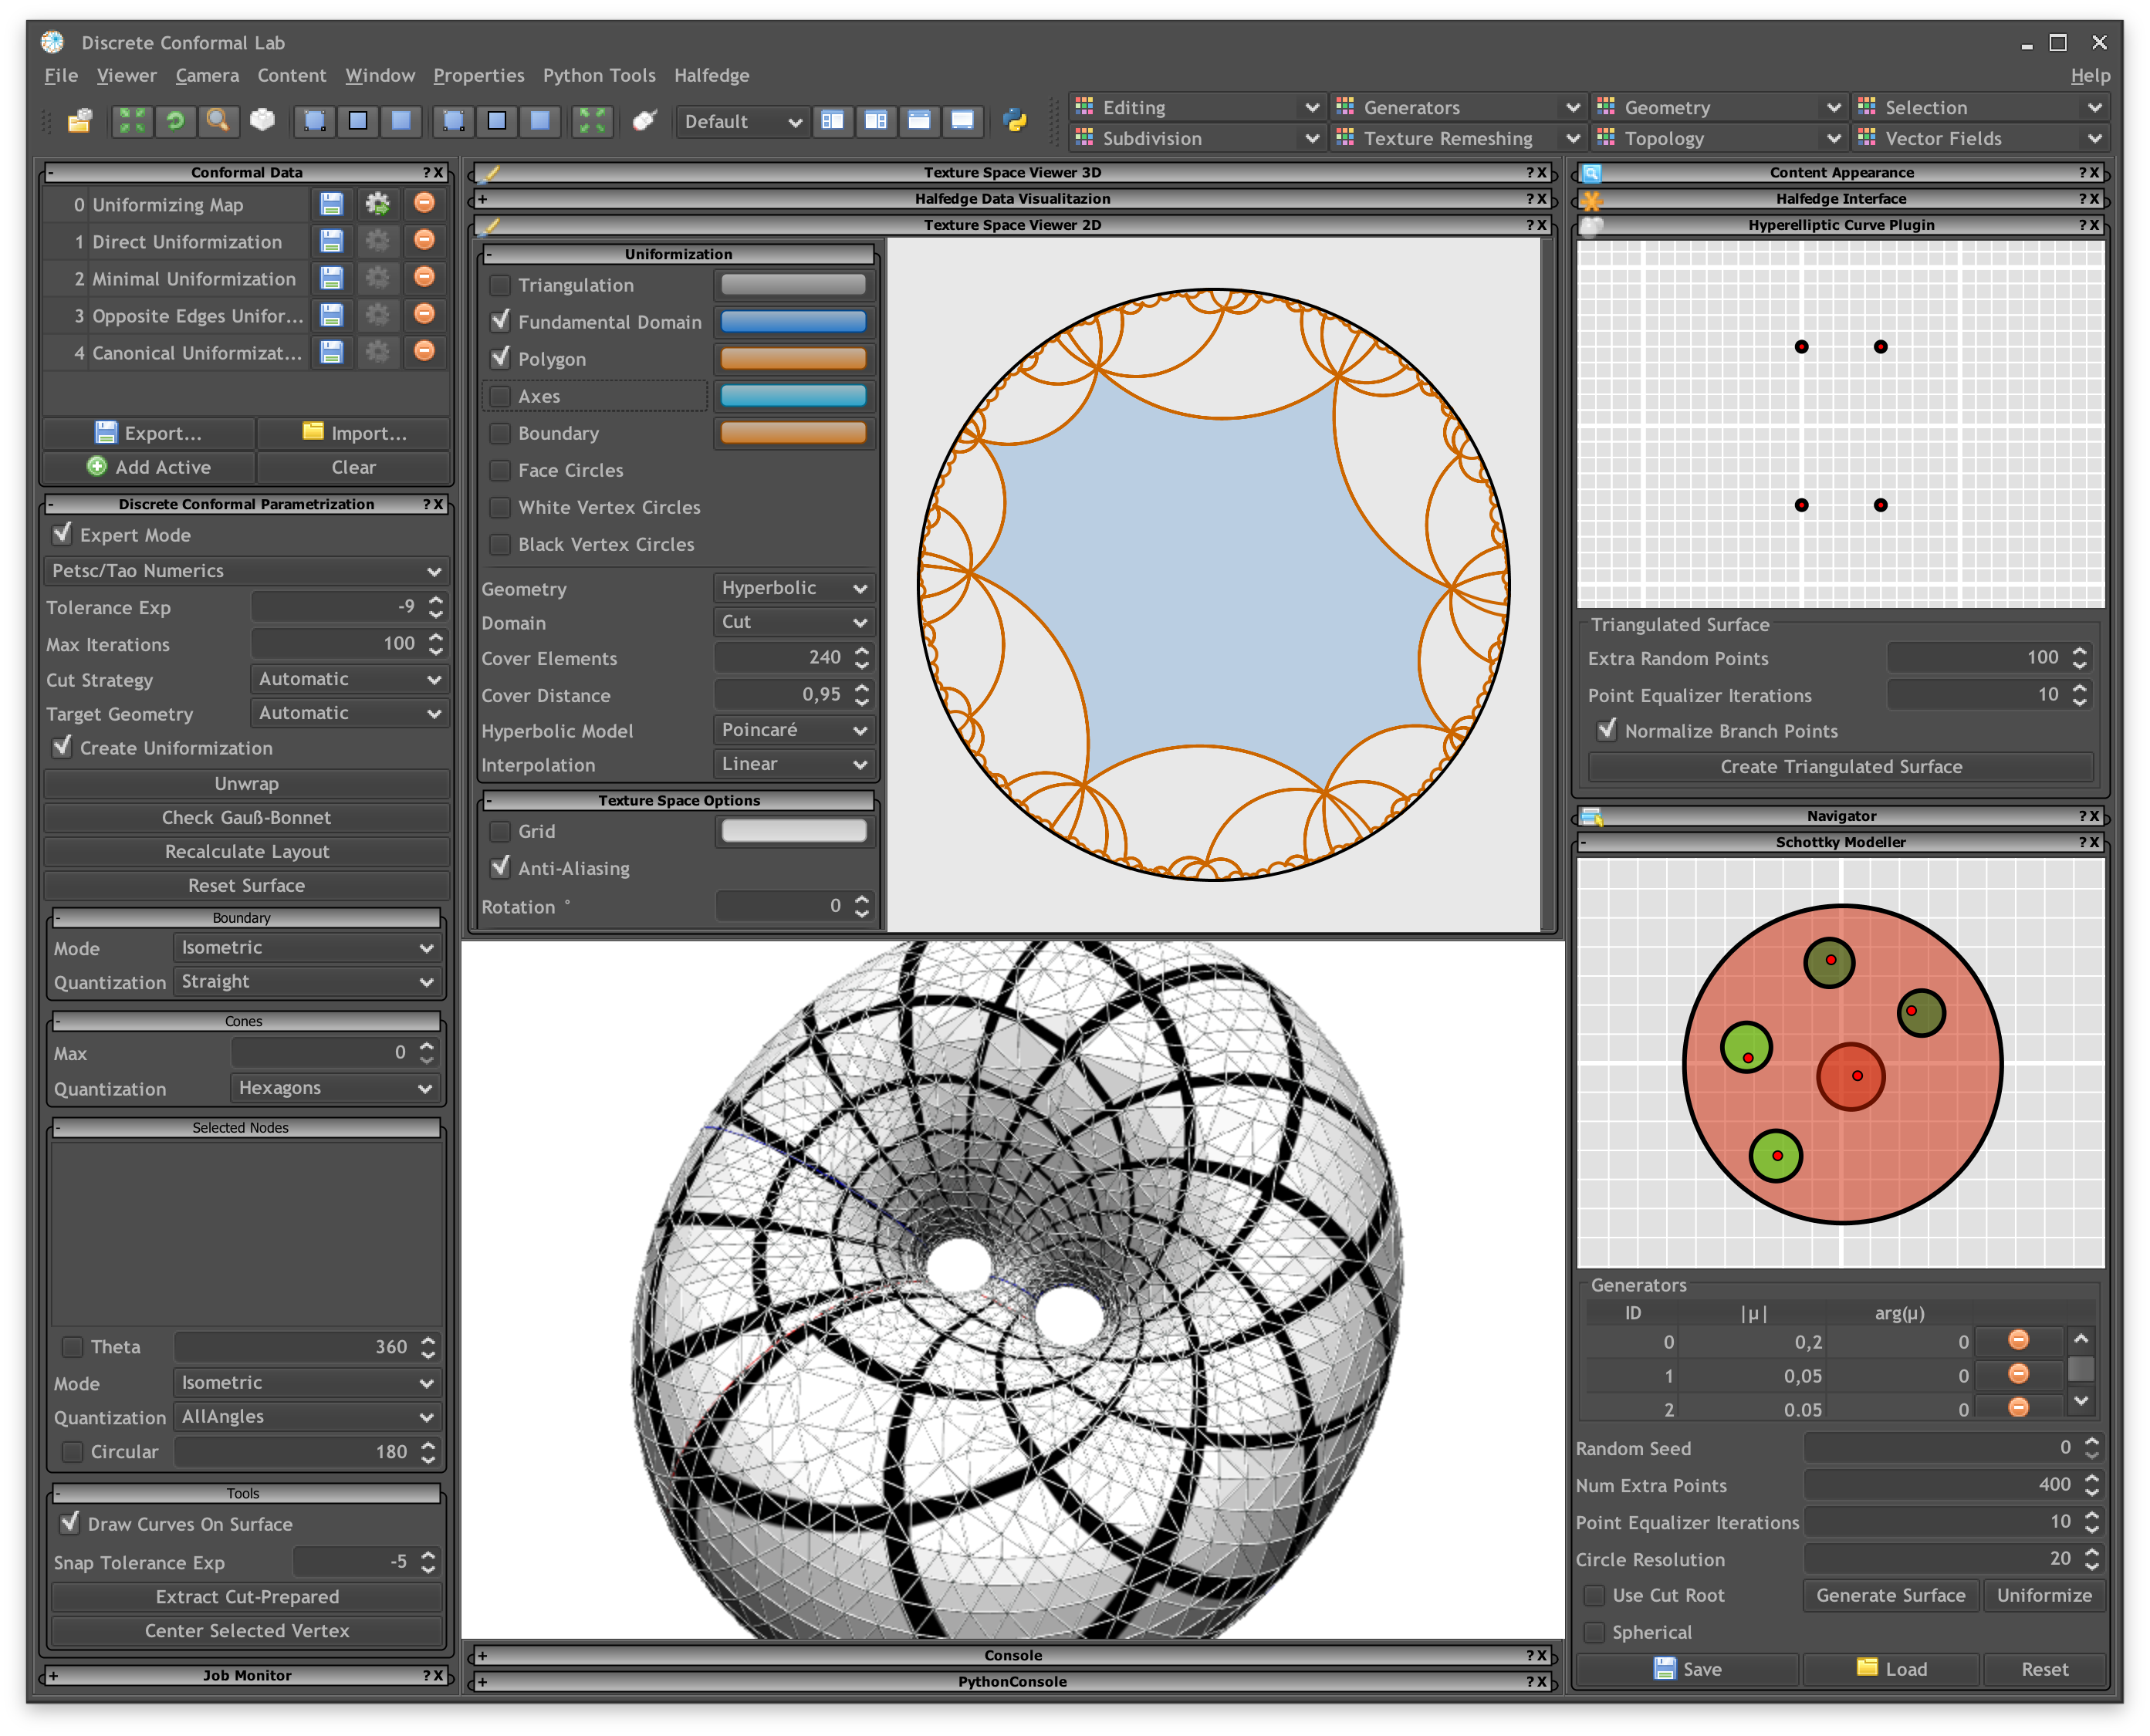
\includegraphics[width=0.7\linewidth]{conformllab/conformallab.png}
\caption{The window of {\sc ConformalLab}.}
\label{fig:conformal_main}
\end{figure}

\section{Data format}
\label{sec:conformal_data}
To store and process data {\sc ConformalLab} uses an {\sc XML} data format.
All examples presented in Chapter~\ref{chp:conformal_examples} are stored
in this format. 
All XML data is contained in the XML namespace 
{\tt http://www.varylab.com/conformallab/types}.


{\bf Schottky data} 

A Riemann surface can be given by Schottky data, see Section~\ref{sec:schottky_examples}. An example is shown in Listing~\ref{lst:schottky_xml}. {\tt SchottkyData} can include one or more {\tt SchottkyGenerator}s. A {\tt SchottkyGenerator} defines fix points $A$ and $B$, the complex number $\mu$, and a {\tt Circle}. This circle is required to contain $A$ and must not contain $B$.

\begin{lstlisting}[label=lst:schottky_xml, caption={A torus given by schotty data}, numbers=none, language=XML, captionpos=b]
<SchottkyData name="Schottky">
	<SchottkyGenerator>
		<A re="-1.0" im="0.0"/>
		<B re="1.0" im="0.0"/>
		<Mu re="0.25" im="0.0"/>
		<Circle radius="1.3">
			<Center re="-1.6" im="0.0"/>
		</Circle>
	</SchottkyGenerator>
</SchottkyData>
\end{lstlisting}

{\bf Hyperelliptic data} 

Hyperelliptic algebraic curves as used in the examples of Section~\ref{sec:examples_elliptic} and \ref{sec:examples_hyperelliptic} are given by the location of their branch points in the complex plane.

\begin{lstlisting}[label=lst:hyperelliptic_xml, caption={A torus given as hyperelliptic data}, numbers=none, language=XML, captionpos=b]
<HyperEllipticAlgebraicCurve name="Curve g2">
	<BranchPoint re="-0.5" im="-1.0"/>
	<BranchPoint re="0.5" im="-1.0"/>
	<BranchPoint re="1.0" im="0.0"/>
	<BranchPoint re="-1.0" im="0.0"/>
</HyperEllipticAlgebraicCurve>
\end{lstlisting}

\begin{lstlisting}[label=lst:hyperelliptic_xml, caption={A torus given as {\tt HalfedegeEmbedding}
with identified edge pairs and vertices.}, numbers=none, language=XML, captionpos=b]
<HalfedgeEmbedding name="Uniformizing Map_domain">
	<Vertex x="0.0" y="0.0" z="0.0" w="1.0" index="0"/>
	<Vertex x="1.0" y="0.0" z="0.0" w="1.0" index="1"/>
	<Vertex x="1.0" y="1.0" z="0.0" w="1.0" index="2"/>
	<Vertex x="0.0" y="1.0" z="0.0" w="1.0" index="3"/>
	<Identification>
		<Vertex>0</Vertex>
		<Vertex>1</Vertex>
		<Vertex>2</Vertex>
		<Vertex>3</Vertex>
	</Identification>
	<Halfedge left="0" target="1" next="1" opposite="4" index="0"/>
	<Halfedge left="0" target="2" next="2" opposite="5" index="1"/>
	<Halfedge left="0" target="3" next="3" opposite="6" index="2"/>
	<Halfedge left="0" target="0" next="0" opposite="7" index="3"/>
	<Halfedge left="-1" target="0" next="7" opposite="0" index="4"/>
	<Halfedge left="-1" target="1" next="4" opposite="1" index="5"/>
	<Halfedge left="-1" target="2" next="5" opposite="2" index="6"/>
	<Halfedge left="-1" target="3" next="6" opposite="3" index="7"/>
	<EdgeIdentification edge1="0" edge2="4" edge3="2" edge4="6"/>
	<EdgeIdentification edge1="1" edge2="5" edge3="3" edge4="7"/>
	<Face index="0"/>
</HalfedgeEmbedding>
\end{lstlisting}

\begin{lstlisting}[label=lst:hyperelliptic_xml, caption={A discrete map is given by a pair of embeddings, the {\tt Domain} and {\tt Image} of the map. Both are of type {\tt HalfedgeEmbedding}.}, numbers=none, language=XML, captionpos=b]
<HalfedgeMap name="Uniformizing Map">
	<Domain name="Uniformizing Map_domain">
		...
	</Domain>
	<Image name="Uniformizing Map_image">
		...
	</Image>
</HalfedgeMap>
\end{lstlisting}

\begin{lstlisting}[label=lst:hyperelliptic_xml, caption={A torus given by its uniformizing group and a fundamental polygon. The elements of the group are either euclidean motions or hyperbolic motions given as elements of $\mathbb PSL_2$.}, numbers=none, language=XML, captionpos=b]
<UniformizationData name="Direct Uniformization">
	<UniformizingGroup>
		<IsometryPSL2R 
			m11="1.0" m12="0.0" m13="1.0" 
			m21="0.0" m22="1.0" m23="0.0" 
			m31="0.0" m32="0.0" m33="1.0"
		/>
		<IsometryPSL2R 
			m11="1.0" m12="0.0" m13="0.0" 
			m21="0.0" m22="1.0" m23="1.0" 
			m31="0.0" m32="0.0" m33="1.0"
		/>
		<IsometryPSL2R 
			m11="1.0" m12="0.0" m13="-1.0" 
			m21="0.0" m22="1.0" m23="0.0" 
			m31="0.0" m32="0.0" m33="1.0"
		/>
		<IsometryPSL2R 
			m11="1.0" m12="0.0" m13="0.0" 
			m21="0.0" m22="1.0" m23="-1.0" 
			m31="0.0" m32="0.0" m33="1.0"
		/>
	</UniformizingGroup>
	<FundamentalPolygon>
		<FundamentalVertex index="0"/>
		<FundamentalEdge index="0" nextEdge="1" previousEdge="3" identifiedEdge="2" startVertex="0">
			<StartPosition re="0.0" im="0.0"/>
		</FundamentalEdge>
		<FundamentalEdge index="1" nextEdge="2" previousEdge="0" identifiedEdge="3" startVertex="0">
			<StartPosition re="1.0" im="0.0"/>
		</FundamentalEdge>
		<FundamentalEdge index="2" nextEdge="3" previousEdge="1" identifiedEdge="0" startVertex="0">
			<StartPosition re="1.0" im="1.0"/>
		</FundamentalEdge>
		<FundamentalEdge index="3" nextEdge="0" previousEdge="2" identifiedEdge="1" startVertex="0">
			<StartPosition re="0.0" im="1.0"/>
		</FundamentalEdge>
	</FundamentalPolygon>
</UniformizationData>
\end{lstlisting}

\begin{lstlisting}[label=lst:hyperelliptic_xml, caption={A wente torus given by a discrete metric. Vertices are given implitly
by following the order of triangle glueings.}, numbers=none, language=XML, captionpos=b]
<DiscreteMetric name="Torus Discrete Metric">
	<MetricEdge length="1.0" index="0"/>
	<MetricEdge length="1.0" index="1"/>
	<MetricEdge length="1.0" index="2"/>
	<MetricEdge length="1.0" index="3"/>
	<MetricEdge length="1.0" index="4"/>
	<MetricEdge length="1.0" index="5"/>
	<MetricEdge length="1.0" index="6"/>
	<MetricEdge length="1.0" index="7"/>
	<MetricEdge length="1.0" index="8"/>
	<MetricEdge length="1.0" index="9"/>
	<MetricEdge length="1.0" index="10"/>
	<MetricEdge length="1.0" index="11"/>
	<MetricTriangle edge1="2" edge2="6" edge3="1"/>
	<MetricTriangle edge1="4" edge2="0" edge3="3"/>
	<MetricTriangle edge1="2" edge2="11" edge3="3"/>
	<MetricTriangle edge1="4" edge2="5" edge3="1"/>
	<MetricTriangle edge1="0" edge2="7" edge3="8"/>
	<MetricTriangle edge1="6" edge2="9" edge3="10"/>
	<MetricTriangle edge1="9" edge2="8" edge3="5"/>
	<MetricTriangle edge1="7" edge2="10" edge3="11"/>
</DiscreteMetric>
\end{lstlisting}


\section{User interface}

The user interface of {\sc ConformalLab} is devided into panels which serve
separate purposes.
\begin{wrapfigure}{R}{0.4\textwidth}
\centering
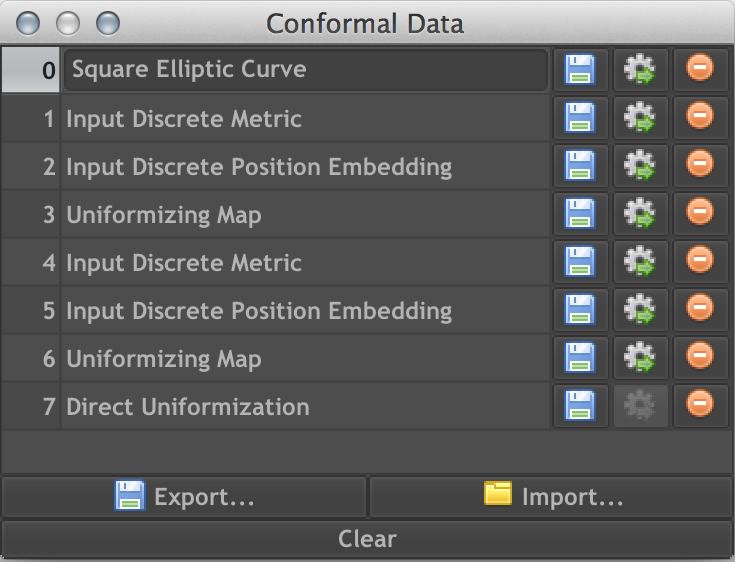
\includegraphics[width=\linewidth]{conformllab/conformal_data.png}
\caption{XML data import and export interface of {\sc ConformalLab}.}
\label{fig:conformal_data}
\end{wrapfigure}
The data import and export panel, see Figure~\ref{fig:conformal_data},
provides functions to import and export data as described in Section~\ref{sec:conformal_data}.
Data can be loaded into memory via the Import button. A table lists the entries of the loaded file.
Loadable are {\tt ConformalDataList} as well as single data instances. The entries of a
{\tt ConformalDataList} are listed in the table of the panel. Each of the rows contains buttons
to save the data to disk (blue disk), load it into the program (gear with green arrow), or delete 
it from the list (red circle).
The function of the load button depends on the data type. A {\tt HalfedgeEmbedding} is
loaded as geometry. A {\tt HalfedgeMap} defined geometry together with texture coordinates
and boundary identifications. If suitable boundary identification is given a uniformizing
group is calculated and visualized.

\begin{wrapfigure}{R}{0.4\textwidth}
\centering
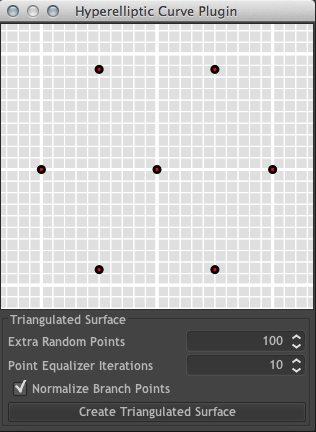
\includegraphics[width=\linewidth]{conformllab/hyperelliptic_curve.png}
\caption{Hyperelliptic curve interface of {\sc ConformalLab}.}
\label{fig:conformal_hyperelliptic}
\end{wrapfigure}

\begin{wrapfigure}{R}{0.4\textwidth}
\centering
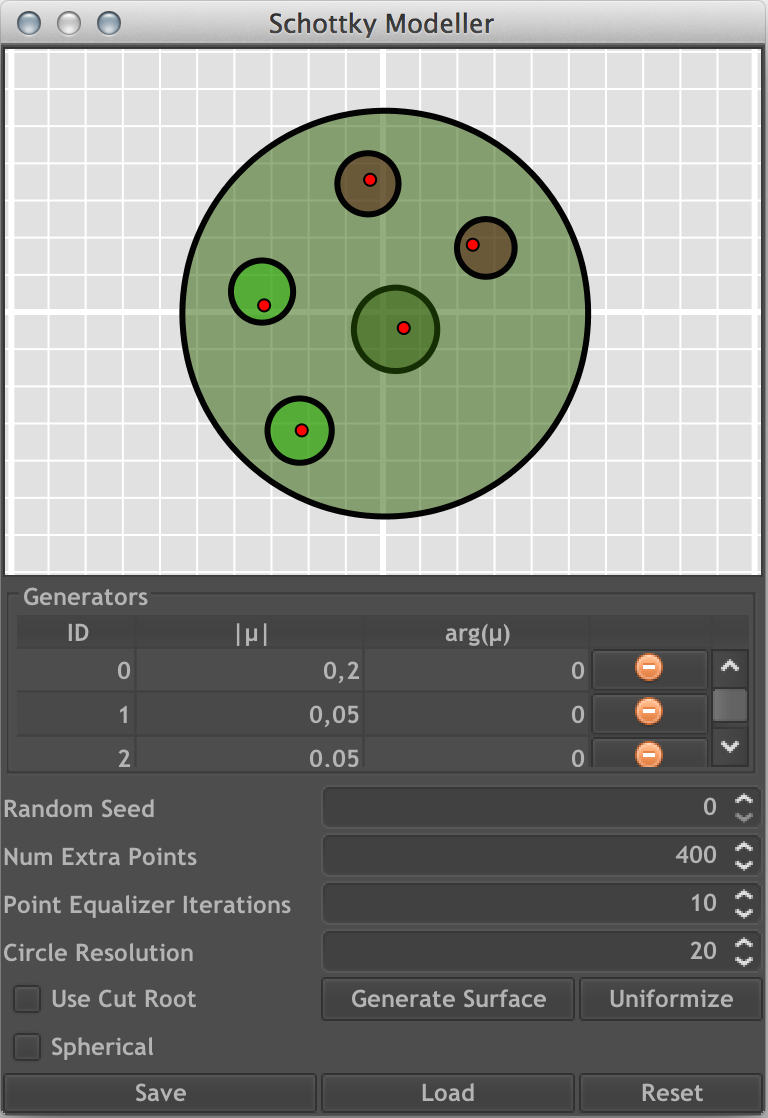
\includegraphics[width=\linewidth]{conformllab/schottky_modeller.png}
\caption{The Schottky modeller user interface of {\sc ConformalLab}.}
\label{fig:conformal_schottky}
\end{wrapfigure}

\begin{wrapfigure}{R}{0.3\textwidth}
\centering
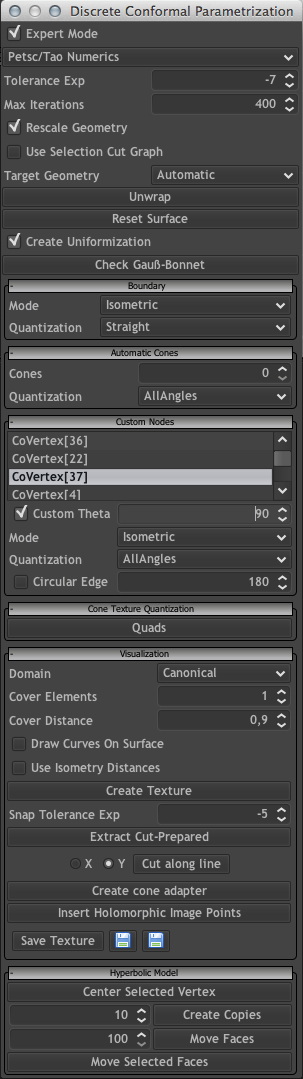
\includegraphics[width=\linewidth]{conformllab/main_interface.png}
\caption{The main interface of {\sc ConformalLab}.}
\label{fig:conformal_main}
\end{wrapfigure}



\subfilebibliography
\end{document}

%%% Local Variables:
%%% TeX-master: "Thesis.tex"
%%% End: